\documentclass[../SWD_disp.tex]{subfiles}

\begin{document}
\section{State Machine Patterns}
State Pattern er et af de 23 GoF patterns. Det hører til kategorien Behavioral Patterns, fordi den definerer måden man kontrollerer kommunikationen mellem klasserne. State Pattern bliver brugt tilm at ændre adfærd på et objekt, når dets interne state bliver ændret.
\\

State Pattern et objekts klasser til, at ændre ved run-time, uden at ændre interfacet der bruges til, at tilgå objektet, eller tabe den nuværende state. Man bruger en context til at skjule ændringerne.

\begin{figure}[H]
    \centering
    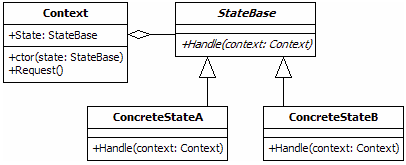
\includegraphics{state_pattern.PNG}
    \caption{State Pattern}
    \label{fig:state_pattern}
\end{figure}

\subsection{Sammenligning: Switch/Case-implementering med GoF State}
State machines har tendens til at blive meget kompliceret. Ofte i advanceret software, skal der skiftes state tit, og det er vigtigt at vide hvilken state man befinder sig i. Derfor er der opfundet et pattern til at hjælpe med det. 
Forstil dig et 4 case switch statement, og hver af disse 4 har yderligere fire har du 256 forksellige states du kan ende i.
Ikke så underligt at der er brugt for et pattern. Det skal så siges, at har du 256 forskellige states at ende i, er det måske på tide at revaluere hele dit design.

Er det ikke så grælt, så kan du bruge state machine pattern

\subsubsection*{Fordele}
\begin{itemize}
    \item Let at udvide med nye states ved at tilføje et objekt (OCP)
    \item Let at sikre at alle metoder bliver udført i de forskellige states da den abstrakte base klasse definerer de metoder.
    \item Let at udvide en states adfærd ved nedarvning fra staten.
\end{itemize}

\subsubsection{Ulemper}
\begin{itemize}
    \item Kode kompleksiteten bliver høj
    \item Svære at se relationerne mellem klasserne, da de er spredt mellem flere forskellige klasser end i switch.
\end{itemize}
\end{document}
